\label{sec:2bound3}

We now have the necessary framework to demonstrate that a closed, oriented 2--manifold bounds a 3--manifold through an explicit construction.
This is useful as a jumping off point for the case one dimension higher, that of 3--manifolds bounding 4--manifolds, which draws on the same framework and methods.

\begin{theorem}
	\label{thm:2bound3}
	Let $\Sigma$ be a closed orientable surface and $f:\Sigma\to[\,0,1\,]$ a proper Morse function with distinct critical values.
	Then there exists a cobordism of the pair $(\Sigma,\emptyset)$ with an explicit handle decomposition described fully by a Stein complex of $f$.
\end{theorem}

\begin{figure}
	\caption{A typical Morse function $T^2\# T^2\to\R$, its Stein factorization, and corresponding dual handle decomposition.}
	\centering
	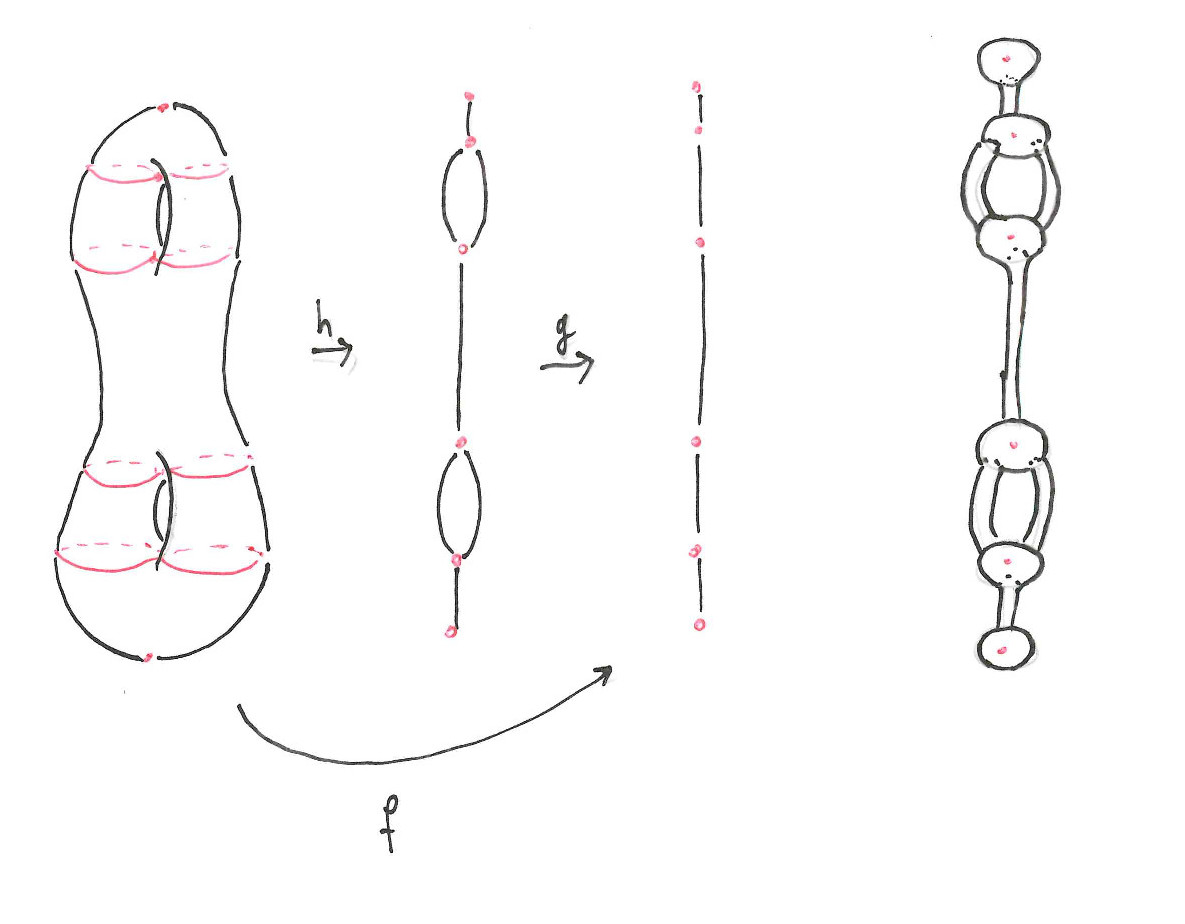
\includegraphics[height=4in]{figures/typicalmorse.jpg}
	\label{fig:typicalmorse}
\end{figure}

\begin{proof}
	Figure \ref{fig:typicalmorse} depicts a typical Morse function acting on the closed oriented surface of genus 2.
	We begin by examining the preimages of points $x\in\R$.
	Denote the space $f\inv(x)$ by $\Sigma_x$, a small interval around $x$ by $\varepsilon(x)=[\,x-\varepsilon,x+\varepsilon\,])$, and the neighbourhood in $\Sigma$ around $\Sigma_x$ by $f\inv(\varepsilon(x))=\varepsilon(\Sigma_x)$.
	The spaces $\Sigma_x$ and $\varepsilon(\Sigma_x)$ may not be connected, so we index the connected components by superscript.
	Let $p$ be a critical point of $f$ with critical value $f(p)=x$.
	By our assumption that critical values are distinct, $p$ is the only critical point of $f$ in $\Sigma_x$.
	The connected component of $\Sigma_x$ containing $p$ is called the \emph{singular fiber} at $p$ and is denoted $\Sigma_x^p$.
	The connected component of $\varepsilon(\Sigma_x)$ containing $p$ is called the \emph{critical neighbourhood} at $p$ and is denoted $\varepsilon^p(\Sigma_x)$.
	
	By the regular value theorem, any regular value pulls back through $f\inv$ to a disjoint collection of circles in $\Sigma$ called \emph{regular fibers}.
	Likewise, a neighbourhood $\varepsilon(x)$ that contains no critical values of $f$ pulls back to a disjoint collection of annuli in $\Sigma$.
	The restriction of $f$ to the components of $\Sigma_x$ that do not contain a critical point has $x$ as a regular value, so the remaining connected components of $\Sigma_x$ are all copies of $S^1$ that we index by $\Sigma_x^i$ for $i=1,\dots,k$, and their associated neighbourhoods are the annuli $\varepsilon^i(\Sigma_x)$.
	When referring to an arbitrary connected subspace of $\Sigma_x$ that could be the singular fiber $\Sigma_x^p$ or a regular fiber $\Sigma_x^i$, we will use the notation $\Sigma_x^*$.
	
	The shape of a singular fiber $\Sigma_x^p$ is determined by the index of $p$.
	Because $f$ is a Morse function whose domain is a surface, its critical points are easily classified by the Morse lemma (Lemma \ref{lem:morselemma}).
	Locally in $\Sigma$, a critical point of index 0 is a minimum, of index 1 a saddle, and of index 2 a maximum.
	
	Let $x$ be a critical value for the critical point $p$ and take $\varepsilon$ to be small enough that $\varepsilon(x)$ contains no critical values other than $x$.
	When $p$ is of index 0 or 2, we can immediately deduce that $\varepsilon^p(\Sigma_x)$ is diffeomorphic to a disc.
	When $p$ is of index 1, the Morse lemma tells us that $\Sigma$ looks like a standard saddle near $p$.
	The intersection of $\Sigma_x^p$ with this saddle is a cross whose centre is $p$.
	For $y\in\varepsilon(x)$, $y$ is a regular value whose preimage is a disjoint union of circles.
	The circles above and below the saddle singularity are the result of smoothing out the cross into a pair of oriented arcs, done in two possible ways.
	The orientations of these circles orient the cross, which has two incoming arms and two outgoing arms which appear in alternating order.
	A Morse function has distinct singular fibers, so the cross we know about in $\Sigma_x^p$ must have its arms connected in $\Sigma_x^p$ through nonsingular orientation--preserving arcs.
	We can then see that $\Sigma_x^p$ is a figure 8, and $\varepsilon^p(\Sigma_x)$ is a pair of pants in $\Sigma$.
	

	\begin{figure}
		\centering
		\caption{Smoothing a cross into a saddle}
		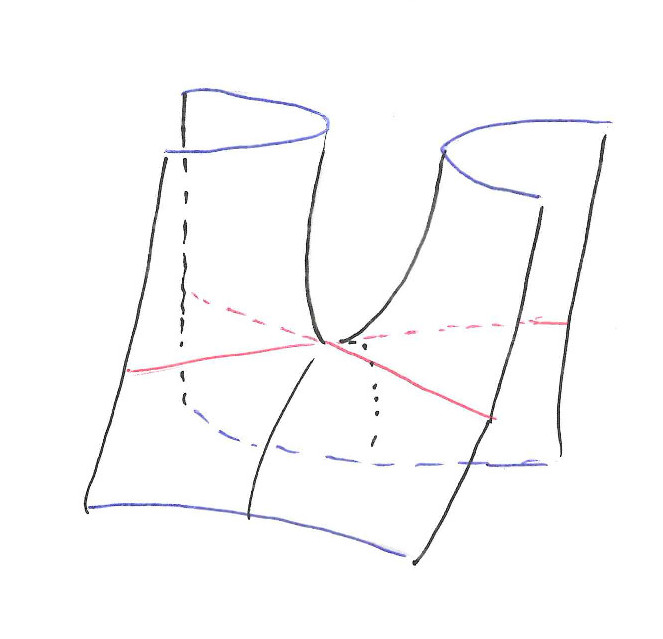
\includegraphics[height=3in]{figures/smoothcross.jpg}
		\label{fig:smoothcross}
	\end{figure}
	
	This analysis is sufficient to form a handle decomposition for a cobordism of $(\Sigma,\emptyset)$.
	We begin with the 3--manifold $\Sigma\times\I$ whose boundary components $\Sigma_0=\Sigma\times\{0\}$ and $\Sigma_1=\Sigma\times\{1\}$ are copies of $\Sigma$, and let $f:\Sigma_0\to\I$ be a Morse function with distinct critical values $x_i$.
	The general idea is that we attach handles to $\Sigma_0$, altering that boundary component until it is empty.
	The $x_i$ partition $\I$ into open intervals containing only regular values.
	We take the associated regular annuli to be attaching regions for 3--dimensional 2--handles, and then fill in what remains with 3--dimensional 3--handles.
	
	For an interval $(x_i,x_{i+1})$, consider the subinterval $\varepsilon(t_i)$ where $x_i<t_i<x_{i+1}$ and $\varepsilon$ is small enough that $\varepsilon(t_i)$ contains neither $x_i$ nor $x_{i+1}$.
	Take the associated regular annuli $\varepsilon(\Sigma_{t_i})$ to be the attaching regions for 3--dimensional 2--handles.
	The boundary component that was once $\Sigma_0$ is now the result of removing the interiors of the annuli $\varepsilon(\Sigma_{t_i})$ from $\Sigma_0$ for each $t_i$, and then introducting discs parallel to the cores of the attached 2--handles.
	These discs are seen as $\DD\times\{0\}$ and $\DD\times\{1\}$ inside of a 2--handle $\DD\times\D^1$.
	The boundary circles of the discs are $\Sigma_{t_i-\varepsilon}$ and $\Sigma_{t_i+\varepsilon}$ for each $i$.
	
	There are now intervals about each critical point that we know, from our analysis above, pull back to discs, annuli, and pairs of pants.
	Each of these subsurfaces have circle boundaries that correspond to the regular fibers $\Sigma_{t_i-\varepsilon}$ and $\Sigma_{t_i+\varepsilon}$ which were capped with discs in the previous step.
	The altered boundary described before is therefore a collection of copies of $S^2$, which we take to be the attaching regions of 3--dimensional 3--handles.
	
	With these handles attached, we obtain $(\Sigma\times\I)\cup\{\textrm{2--handles}\}\cup\{\textrm{3--handles}\}$, which is a 3--manifold whose only boundary component is $\Sigma_1$, i.e. is a cobordism of the pair $(\Sigma,\emptyset)$.
	
	The corresponding dual handle decomposition is realized by turning the process upside down.
	Where we previously had 3--handle attachments with cores $\D^3\times\{\vec{0}\}$ and cocores $\{\vec{0}\}\times\{\vec{0}\}$, we now have 0--handles with cores $\{\vec{0}\}\times\{\vec{0}\}$ and cocores $\D^3\times\{\vec{0}\}$.
	In other words, the dual construction begins by taking the disjoint union of a collection of 3--discs that correspond to the space obtained by capping the boundary circles of the components $\varepsilon(\Sigma_{x_i})$ with 2--discs and then filling the spheres with 3--balls.
	Where we previously had 2--handle attachments with cores $\DD\times\{\vec{0}\}$ and cocores $\{\vec{0}\}\times\D^1$, we now have 1--handle attachments with cores $\{\vec{0}\}\times\D^1$ and cocores $\DD\times\{\vec{0}\}$.
	In other words, we connect the 0--handles together using 1--handles.
	The old belt 0--spheres of the 2--handles in the previous construction correspond here to new attaching 0--spheres, and the attaching maps are chosen to preserve orientability cf.\ Remark~\ref{rmk:1handle}.
	The new attaching 0--spheres bound the new cores, the old core 2--discs are now cocores.
	This construction yields a 3--manifold whose boundary is exactly $\Sigma$, and is indeed another cobordism of the pair $(\Sigma,\emptyset)$.
	
	A Stein factorization $f=g\comp h$ is simple to describe.
	Define the equivalence relation $\sim$ on the points in $\Sigma$ by putting $p\sim q$ if and only if $f(p)=f(q)=x$ and $p$ and $q$ are in the same subspace $\Sigma_x^*$.
	Then $h$ is the quotient map $\Sigma\to \Sigma/\!\!\sim$ where the points of $\Sigma/\!\!\sim$ are the subspaces $\Sigma_x^*$, and $g$ is the map $\Sigma/\!\!\sim\, \to\R$ defined by $g(\Sigma_x^*)=x$.

	The Stein complex $S=\Sigma/\!\!\sim$ can be viewed as a graph $G$.
	A critical value $x=f(p)$ has as its preimage one associated singular fiber $\Sigma_x^p$ in $S$ plus a number of copies of $S^1$ (possibly 0) given by $\Sigma_x^i$.
	We take the associated points $h(\Sigma_x)$ in $S$ for each critical value to be the vertex set $v(G)$.
	For a pair of adjacent critical values $x_{j}$, $x_{j+1}$, an appropriate choice of $\varepsilon$ and $x\in(x_{j},x_{j+1})$ yields a collection of regular annuli $\varepsilon(\Sigma_x)$ in $\Sigma$ that has boundary inside of $\Sigma_{x_{j}}\cup\Sigma_{x_{j+1}}$.
	In $S$, we find $h(\varepsilon(\Sigma_x))$ to consist of 1--dimensional strands that connect components of $\Sigma_{x_{j}}$ and $\Sigma_{x_{j+1}}$.
	The set of pairs $(v,w)$ of connected subspaces with $v\in\Sigma_{x_{j}}$ and $w\in\Sigma_{x_{j+1}}$ such that $v$ and $w$ are connected by a strand in $S$ forms the edge set $e(G)$.
	
	At this point, $G$ corresponds exactly to the dual handle decomposition given earlier.
	For each vertex of $G$ we get a 0--handle.
	For each edge, a 1--handle.
	We attach 1--handles with only one demand: that the resulting space continues to be orientable.
\end{proof}

The Stein complex obtained in the proof of Theorem~\ref{thm:2bound3} may have superfluous vertices.
In particular, a vertex $v$ of $G$ that is adjacent to exactly two verticex $u$ and $w$ via the edges $(u,v)$ and $(v,w)$ may be replaced, along with its adjacent edges, by a single edge $(u,w)$.
To see that the handle decomposition described by this Stein complex graph is equivalent, examine the attaching region of the 1--handle corresponding to $(u,v)$ as it sits inside the boundary of the 0--handle corresponding to $v$.
This region may be isotoped over the 1--handle corresponding to $(v,w)$, where it ends up in the boundary of the 0--handle corresponding to $w$.
We are left with a 0--handle $v$ and 1--handle $(v,w)$ that are contractible into $w$.